\documentclass[twoside]{book}

% Packages required by doxygen
\usepackage{fixltx2e}
\usepackage{calc}
\usepackage{doxygen}
\usepackage[export]{adjustbox} % also loads graphicx
\usepackage{graphicx}
\usepackage[utf8]{inputenc}
\usepackage{makeidx}
\usepackage{multicol}
\usepackage{multirow}
\PassOptionsToPackage{warn}{textcomp}
\usepackage{textcomp}
\usepackage[nointegrals]{wasysym}
\usepackage[table]{xcolor}

% Font selection
\usepackage[T1]{fontenc}
\usepackage[scaled=.90]{helvet}
\usepackage{courier}
\usepackage{amssymb}
\usepackage{sectsty}
\renewcommand{\familydefault}{\sfdefault}
\allsectionsfont{%
  \fontseries{bc}\selectfont%
  \color{darkgray}%
}
\renewcommand{\DoxyLabelFont}{%
  \fontseries{bc}\selectfont%
  \color{darkgray}%
}
\newcommand{\+}{\discretionary{\mbox{\scriptsize$\hookleftarrow$}}{}{}}

% Page & text layout
\usepackage{geometry}
\geometry{%
  a4paper,%
  top=2.5cm,%
  bottom=2.5cm,%
  left=2.5cm,%
  right=2.5cm%
}
\tolerance=750
\hfuzz=15pt
\hbadness=750
\setlength{\emergencystretch}{15pt}
\setlength{\parindent}{0cm}
\setlength{\parskip}{3ex plus 2ex minus 2ex}
\makeatletter
\renewcommand{\paragraph}{%
  \@startsection{paragraph}{4}{0ex}{-1.0ex}{1.0ex}{%
    \normalfont\normalsize\bfseries\SS@parafont%
  }%
}
\renewcommand{\subparagraph}{%
  \@startsection{subparagraph}{5}{0ex}{-1.0ex}{1.0ex}{%
    \normalfont\normalsize\bfseries\SS@subparafont%
  }%
}
\makeatother

% Headers & footers
\usepackage{fancyhdr}
\pagestyle{fancyplain}
\fancyhead[LE]{\fancyplain{}{\bfseries\thepage}}
\fancyhead[CE]{\fancyplain{}{}}
\fancyhead[RE]{\fancyplain{}{\bfseries\leftmark}}
\fancyhead[LO]{\fancyplain{}{\bfseries\rightmark}}
\fancyhead[CO]{\fancyplain{}{}}
\fancyhead[RO]{\fancyplain{}{\bfseries\thepage}}
\fancyfoot[LE]{\fancyplain{}{}}
\fancyfoot[CE]{\fancyplain{}{}}
\fancyfoot[RE]{\fancyplain{}{\bfseries\scriptsize Generated by Doxygen }}
\fancyfoot[LO]{\fancyplain{}{\bfseries\scriptsize Generated by Doxygen }}
\fancyfoot[CO]{\fancyplain{}{}}
\fancyfoot[RO]{\fancyplain{}{}}
\renewcommand{\footrulewidth}{0.4pt}
\renewcommand{\chaptermark}[1]{%
  \markboth{#1}{}%
}
\renewcommand{\sectionmark}[1]{%
  \markright{\thesection\ #1}%
}

% Indices & bibliography
\usepackage{natbib}
\usepackage[titles]{tocloft}
\setcounter{tocdepth}{3}
\setcounter{secnumdepth}{5}
\makeindex

% Hyperlinks (required, but should be loaded last)
\usepackage{ifpdf}
\ifpdf
  \usepackage[pdftex,pagebackref=true]{hyperref}
\else
  \usepackage[ps2pdf,pagebackref=true]{hyperref}
\fi
\hypersetup{%
  colorlinks=true,%
  linkcolor=blue,%
  citecolor=blue,%
  unicode%
}

% Custom commands
\newcommand{\clearemptydoublepage}{%
  \newpage{\pagestyle{empty}\cleardoublepage}%
}

\usepackage{caption}
\captionsetup{labelsep=space,justification=centering,font={bf},singlelinecheck=off,skip=4pt,position=top}

%===== C O N T E N T S =====

\begin{document}

% Titlepage & ToC
\hypersetup{pageanchor=false,
             bookmarksnumbered=true,
             pdfencoding=unicode
            }
\pagenumbering{alph}
\begin{titlepage}
\vspace*{7cm}
\begin{center}%
{\Large My Project }\\
\vspace*{1cm}
{\large Generated by Doxygen 1.8.13}\\
\end{center}
\end{titlepage}
\clearemptydoublepage
\pagenumbering{roman}
\tableofcontents
\clearemptydoublepage
\pagenumbering{arabic}
\hypersetup{pageanchor=true}

%--- Begin generated contents ---
\chapter{Class Index}
\section{Class List}
Here are the classes, structs, unions and interfaces with brief descriptions\+:\begin{DoxyCompactList}
\item\contentsline{section}{\hyperlink{structAnimatedSprite}{Animated\+Sprite} }{\pageref{structAnimatedSprite}}{}
\item\contentsline{section}{\hyperlink{structBackground}{Background} }{\pageref{structBackground}}{}
\item\contentsline{section}{\hyperlink{structjoueur}{joueur} }{\pageref{structjoueur}}{}
\item\contentsline{section}{\hyperlink{structminibox}{minibox} }{\pageref{structminibox}}{}
\item\contentsline{section}{\hyperlink{structMinimap}{Minimap} }{\pageref{structMinimap}}{}
\item\contentsline{section}{\hyperlink{structPlayerScore}{Player\+Score} }{\pageref{structPlayerScore}}{}
\item\contentsline{section}{\hyperlink{structprojectile}{projectile} }{\pageref{structprojectile}}{}
\end{DoxyCompactList}

\chapter{Class Documentation}
\hypertarget{structAnimatedSprite}{}\section{Animated\+Sprite Struct Reference}
\label{structAnimatedSprite}\index{Animated\+Sprite@{Animated\+Sprite}}
\subsection*{Public Attributes}
\begin{DoxyCompactItemize}
\item 
\mbox{\Hypertarget{structAnimatedSprite_a27cb96c65de531dad610ae4874479a33}\label{structAnimatedSprite_a27cb96c65de531dad610ae4874479a33}} 
S\+D\+L\+\_\+\+Surface $\ast$ {\bfseries spritesheet}
\item 
\mbox{\Hypertarget{structAnimatedSprite_ad78cd918a5b05a95beb286e6b6d138e4}\label{structAnimatedSprite_ad78cd918a5b05a95beb286e6b6d138e4}} 
S\+D\+L\+\_\+\+Rect {\bfseries clips} \mbox{[}T\+O\+T\+A\+L\+\_\+\+F\+R\+A\+M\+ES\mbox{]}
\item 
\mbox{\Hypertarget{structAnimatedSprite_a59bce95aa316e3a327a96dcd1fe945b3}\label{structAnimatedSprite_a59bce95aa316e3a327a96dcd1fe945b3}} 
int {\bfseries current\+\_\+frame}
\item 
\mbox{\Hypertarget{structAnimatedSprite_ac24913de61be8e53c0b63acb58b30ca9}\label{structAnimatedSprite_ac24913de61be8e53c0b63acb58b30ca9}} 
Uint32 {\bfseries last\+\_\+frame\+\_\+time}
\item 
\mbox{\Hypertarget{structAnimatedSprite_aac6b3af9fd7075bdef303c025b5a2035}\label{structAnimatedSprite_aac6b3af9fd7075bdef303c025b5a2035}} 
Uint32 {\bfseries frame\+\_\+delay}
\item 
\mbox{\Hypertarget{structAnimatedSprite_ae0e283c0401edea10ed6a7dd46a7296e}\label{structAnimatedSprite_ae0e283c0401edea10ed6a7dd46a7296e}} 
int {\bfseries facing\+Left}
\end{DoxyCompactItemize}


The documentation for this struct was generated from the following file\+:\begin{DoxyCompactItemize}
\item 
header.\+h\end{DoxyCompactItemize}

\hypertarget{structBackground}{}\section{Background Struct Reference}
\label{structBackground}\index{Background@{Background}}
\subsection*{Public Attributes}
\begin{DoxyCompactItemize}
\item 
\mbox{\Hypertarget{structBackground_a7e2ff64dc25f84e6be445bbfffd0217e}\label{structBackground_a7e2ff64dc25f84e6be445bbfffd0217e}} 
S\+D\+L\+\_\+\+Surface $\ast$ {\bfseries bg1}
\item 
\mbox{\Hypertarget{structBackground_a1a5ed8c454159592cce738937e90970b}\label{structBackground_a1a5ed8c454159592cce738937e90970b}} 
S\+D\+L\+\_\+\+Surface $\ast$ {\bfseries bg2}
\item 
\mbox{\Hypertarget{structBackground_a10213a83c3d22a8b8617f202758a6001}\label{structBackground_a10213a83c3d22a8b8617f202758a6001}} 
S\+D\+L\+\_\+\+Rect {\bfseries camera1}
\item 
\mbox{\Hypertarget{structBackground_a4d756b04725d0079bd2b7647a684b652}\label{structBackground_a4d756b04725d0079bd2b7647a684b652}} 
S\+D\+L\+\_\+\+Rect {\bfseries camera2}
\item 
\mbox{\Hypertarget{structBackground_a55a1f4f519ef08adfb861f259d4770e8}\label{structBackground_a55a1f4f519ef08adfb861f259d4770e8}} 
S\+D\+L\+\_\+\+Rect {\bfseries camera\+Solo}
\item 
\mbox{\Hypertarget{structBackground_a50c75fc3176420a9941167b6b2a30dcd}\label{structBackground_a50c75fc3176420a9941167b6b2a30dcd}} 
S\+D\+L\+\_\+\+Rect {\bfseries pos\+Ecran1}
\item 
\mbox{\Hypertarget{structBackground_a0446f53696f1a9b0fc466de5683f335d}\label{structBackground_a0446f53696f1a9b0fc466de5683f335d}} 
S\+D\+L\+\_\+\+Rect {\bfseries pos\+Ecran2}
\end{DoxyCompactItemize}


The documentation for this struct was generated from the following file\+:\begin{DoxyCompactItemize}
\item 
background.\+h\end{DoxyCompactItemize}

\hypertarget{structjoueur}{}\section{joueur Struct Reference}
\label{structjoueur}\index{joueur@{joueur}}
\subsection*{Public Attributes}
\begin{DoxyCompactItemize}
\item 
\mbox{\Hypertarget{structjoueur_ae9a49531bc2f35918bbc646718d14f53}\label{structjoueur_ae9a49531bc2f35918bbc646718d14f53}} 
S\+D\+L\+\_\+\+Surface $\ast$ {\bfseries sprites} \mbox{[}8\mbox{]}
\item 
\mbox{\Hypertarget{structjoueur_ac37866aa94ec0ee62d729b627293340e}\label{structjoueur_ac37866aa94ec0ee62d729b627293340e}} 
S\+D\+L\+\_\+\+Surface $\ast$ {\bfseries image}
\item 
\mbox{\Hypertarget{structjoueur_acb1caaddeb22f11809e05fa2b90c4d4d}\label{structjoueur_acb1caaddeb22f11809e05fa2b90c4d4d}} 
S\+D\+L\+\_\+\+Surface $\ast$ {\bfseries vie} \mbox{[}10\mbox{]}
\item 
\mbox{\Hypertarget{structjoueur_a00972395a785d67166f9997cb75e93aa}\label{structjoueur_a00972395a785d67166f9997cb75e93aa}} 
S\+D\+L\+\_\+\+Surface $\ast$ {\bfseries score}
\item 
\mbox{\Hypertarget{structjoueur_a490dc132329c3040775237d6d76c468d}\label{structjoueur_a490dc132329c3040775237d6d76c468d}} 
S\+D\+L\+\_\+\+Rect {\bfseries frame}
\item 
\mbox{\Hypertarget{structjoueur_aa523fc8c3537f0cc97be75ff9fca19e1}\label{structjoueur_aa523fc8c3537f0cc97be75ff9fca19e1}} 
int {\bfseries current\+\_\+frame}
\item 
\mbox{\Hypertarget{structjoueur_a48fdd16e51d3c64b58ffa4b337d4c822}\label{structjoueur_a48fdd16e51d3c64b58ffa4b337d4c822}} 
int {\bfseries animation\+\_\+state}
\item 
\mbox{\Hypertarget{structjoueur_a0a698a48320cbc327a934d242d66d72c}\label{structjoueur_a0a698a48320cbc327a934d242d66d72c}} 
Uint32 {\bfseries frame\+\_\+timer}
\item 
\mbox{\Hypertarget{structjoueur_aa9133278174ad13c6de1d0675c77adc6}\label{structjoueur_aa9133278174ad13c6de1d0675c77adc6}} 
int {\bfseries facing}
\item 
\mbox{\Hypertarget{structjoueur_a0df959136c568eefc862c620e42098a7}\label{structjoueur_a0df959136c568eefc862c620e42098a7}} 
S\+D\+L\+\_\+\+Rect {\bfseries posV} \mbox{[}10\mbox{]}
\item 
\mbox{\Hypertarget{structjoueur_a54599e8b1af93435eadff40780751a53}\label{structjoueur_a54599e8b1af93435eadff40780751a53}} 
S\+D\+L\+\_\+\+Rect {\bfseries posS}
\item 
\mbox{\Hypertarget{structjoueur_a9390dbbfe56dcfed1303ebb3a8eb4464}\label{structjoueur_a9390dbbfe56dcfed1303ebb3a8eb4464}} 
S\+D\+L\+\_\+\+Rect {\bfseries pos}
\item 
\mbox{\Hypertarget{structjoueur_ad33e581f9d930071a4d8255026e19730}\label{structjoueur_ad33e581f9d930071a4d8255026e19730}} 
float {\bfseries x\+\_\+vit}
\item 
\mbox{\Hypertarget{structjoueur_af1e2def44f8968de5acec0eb534f1aaa}\label{structjoueur_af1e2def44f8968de5acec0eb534f1aaa}} 
float {\bfseries y\+\_\+vit}
\item 
\mbox{\Hypertarget{structjoueur_aa81fe7a9557e034692a9acd17bcb3c66}\label{structjoueur_aa81fe7a9557e034692a9acd17bcb3c66}} 
int {\bfseries life\+\_\+count}
\item 
\mbox{\Hypertarget{structjoueur_ae429ab2b1383c4d404f2912ba14a653a}\label{structjoueur_ae429ab2b1383c4d404f2912ba14a653a}} 
int {\bfseries score\+\_\+count}
\end{DoxyCompactItemize}


The documentation for this struct was generated from the following file\+:\begin{DoxyCompactItemize}
\item 
header.\+h\end{DoxyCompactItemize}

\hypertarget{structminibox}{}\section{minibox Struct Reference}
\label{structminibox}\index{minibox@{minibox}}


Collaboration diagram for minibox\+:
\nopagebreak
\begin{figure}[H]
\begin{center}
\leavevmode
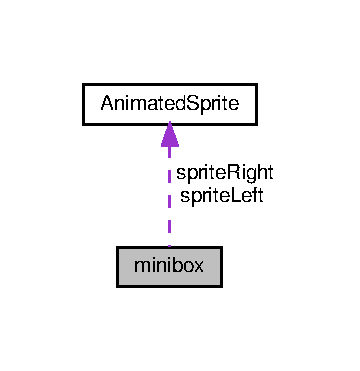
\includegraphics[width=173pt]{structminibox__coll__graph}
\end{center}
\end{figure}
\subsection*{Public Attributes}
\begin{DoxyCompactItemize}
\item 
\mbox{\Hypertarget{structminibox_a571c9e29b790d024f8cfd0642190744b}\label{structminibox_a571c9e29b790d024f8cfd0642190744b}} 
S\+D\+L\+\_\+\+Surface $\ast$ {\bfseries surface}
\item 
\mbox{\Hypertarget{structminibox_ac21698b8e91affc5bb381d48327d16d5}\label{structminibox_ac21698b8e91affc5bb381d48327d16d5}} 
S\+D\+L\+\_\+\+Rect {\bfseries rect}
\item 
\mbox{\Hypertarget{structminibox_a0f15ad467c6be08d84d9babd9439dbfa}\label{structminibox_a0f15ad467c6be08d84d9babd9439dbfa}} 
int {\bfseries xvitesse}
\item 
\mbox{\Hypertarget{structminibox_a340d9ec37887abc1a2732c7a0076bd6c}\label{structminibox_a340d9ec37887abc1a2732c7a0076bd6c}} 
int {\bfseries yvitesse}
\item 
\mbox{\Hypertarget{structminibox_acf849c664f51543a5afacb8233d669c0}\label{structminibox_acf849c664f51543a5afacb8233d669c0}} 
int {\bfseries xacc}
\item 
\mbox{\Hypertarget{structminibox_a75753c3958c711f9b272fbbc51aea2c9}\label{structminibox_a75753c3958c711f9b272fbbc51aea2c9}} 
int {\bfseries yacc}
\item 
\mbox{\Hypertarget{structminibox_a73355ddfc131585fec6aed49d4168e49}\label{structminibox_a73355ddfc131585fec6aed49d4168e49}} 
int {\bfseries accident}
\item 
\mbox{\Hypertarget{structminibox_a6fe4a0b46bd6f862db774085dcc3f42e}\label{structminibox_a6fe4a0b46bd6f862db774085dcc3f42e}} 
int {\bfseries sante}
\item 
\mbox{\Hypertarget{structminibox_a685e2bbceba1d7c6d5b82ba67288b1cd}\label{structminibox_a685e2bbceba1d7c6d5b82ba67288b1cd}} 
Enemy\+State {\bfseries state}
\item 
\mbox{\Hypertarget{structminibox_ac33fd0e8b9e74d1e48ebe6161f6b1b58}\label{structminibox_ac33fd0e8b9e74d1e48ebe6161f6b1b58}} 
int {\bfseries patrol\+\_\+dir}
\item 
\mbox{\Hypertarget{structminibox_a11e514c3b24e290dc90c92f3bef45c43}\label{structminibox_a11e514c3b24e290dc90c92f3bef45c43}} 
int {\bfseries facing\+Left}
\item 
\mbox{\Hypertarget{structminibox_a4a90e5b68bea0bcedee6b60b810b342f}\label{structminibox_a4a90e5b68bea0bcedee6b60b810b342f}} 
\hyperlink{structAnimatedSprite}{Animated\+Sprite} {\bfseries sprite\+Right}
\item 
\mbox{\Hypertarget{structminibox_a406076968790710a0f03e76455239fd6}\label{structminibox_a406076968790710a0f03e76455239fd6}} 
\hyperlink{structAnimatedSprite}{Animated\+Sprite} {\bfseries sprite\+Left}
\item 
\mbox{\Hypertarget{structminibox_a145b58a92d721ede3f4013cdc7dd30ba}\label{structminibox_a145b58a92d721ede3f4013cdc7dd30ba}} 
int {\bfseries chase}
\end{DoxyCompactItemize}


The documentation for this struct was generated from the following file\+:\begin{DoxyCompactItemize}
\item 
header.\+h\end{DoxyCompactItemize}

\hypertarget{structMinimap}{}\section{Minimap Struct Reference}
\label{structMinimap}\index{Minimap@{Minimap}}
\subsection*{Public Attributes}
\begin{DoxyCompactItemize}
\item 
\mbox{\Hypertarget{structMinimap_ae1792d7a5459227ec30b7c1e84a586fc}\label{structMinimap_ae1792d7a5459227ec30b7c1e84a586fc}} 
S\+D\+L\+\_\+\+Surface $\ast$ {\bfseries image}
\item 
\mbox{\Hypertarget{structMinimap_a73ac826eda03036d5155107a3f09c859}\label{structMinimap_a73ac826eda03036d5155107a3f09c859}} 
S\+D\+L\+\_\+\+Surface $\ast$ {\bfseries point}
\item 
\mbox{\Hypertarget{structMinimap_aef71ccf7b909205b833a1f0a2e35ab2c}\label{structMinimap_aef71ccf7b909205b833a1f0a2e35ab2c}} 
S\+D\+L\+\_\+\+Rect {\bfseries position\+Image}
\item 
\mbox{\Hypertarget{structMinimap_a5de6d582e4ddfb33bd6a67576f597893}\label{structMinimap_a5de6d582e4ddfb33bd6a67576f597893}} 
S\+D\+L\+\_\+\+Rect {\bfseries position\+Point}
\item 
\mbox{\Hypertarget{structMinimap_a8dc5018c4e90d5dd04ce7de5fbcf30c3}\label{structMinimap_a8dc5018c4e90d5dd04ce7de5fbcf30c3}} 
int {\bfseries largeur\+Fond}
\item 
\mbox{\Hypertarget{structMinimap_a3d158a9ddb6bbf9764680b7a0a7258ff}\label{structMinimap_a3d158a9ddb6bbf9764680b7a0a7258ff}} 
int {\bfseries hauteur\+Fond}
\item 
\mbox{\Hypertarget{structMinimap_a6464a8fa9809cc4ab048058b43380bfc}\label{structMinimap_a6464a8fa9809cc4ab048058b43380bfc}} 
int {\bfseries largeur\+Minimap}
\item 
\mbox{\Hypertarget{structMinimap_a449245f57db6d6164fb6bf552a010576}\label{structMinimap_a449245f57db6d6164fb6bf552a010576}} 
int {\bfseries hauteur\+Minimap}
\end{DoxyCompactItemize}


The documentation for this struct was generated from the following file\+:\begin{DoxyCompactItemize}
\item 
minimap.\+h\end{DoxyCompactItemize}

\hypertarget{structPlayerScore}{}\section{Player\+Score Struct Reference}
\label{structPlayerScore}\index{Player\+Score@{Player\+Score}}
\subsection*{Public Attributes}
\begin{DoxyCompactItemize}
\item 
\mbox{\Hypertarget{structPlayerScore_af8a049451b4b160d55b9494faa1156d2}\label{structPlayerScore_af8a049451b4b160d55b9494faa1156d2}} 
char {\bfseries name} \mbox{[}256\mbox{]}
\item 
\mbox{\Hypertarget{structPlayerScore_ace29a1b82acd6d4fdcc6398c93131141}\label{structPlayerScore_ace29a1b82acd6d4fdcc6398c93131141}} 
int {\bfseries score}
\end{DoxyCompactItemize}


The documentation for this struct was generated from the following files\+:\begin{DoxyCompactItemize}
\item 
meilleur.\+c\item 
meilleur.\+h\end{DoxyCompactItemize}

\hypertarget{structprojectile}{}\section{projectile Struct Reference}
\label{structprojectile}\index{projectile@{projectile}}
\subsection*{Public Attributes}
\begin{DoxyCompactItemize}
\item 
\mbox{\Hypertarget{structprojectile_acbb67899abcc06c86f8747f2059db168}\label{structprojectile_acbb67899abcc06c86f8747f2059db168}} 
S\+D\+L\+\_\+\+Surface $\ast$ {\bfseries surface}
\item 
\mbox{\Hypertarget{structprojectile_a450e7ca8a05fe4043a63e73b88f4c7a9}\label{structprojectile_a450e7ca8a05fe4043a63e73b88f4c7a9}} 
S\+D\+L\+\_\+\+Rect {\bfseries rect}
\item 
\mbox{\Hypertarget{structprojectile_aa84ac35cbc967bee2b13a4d31ff11360}\label{structprojectile_aa84ac35cbc967bee2b13a4d31ff11360}} 
int {\bfseries active}
\item 
\mbox{\Hypertarget{structprojectile_aa2af53bce63feecb719ef1edba54689e}\label{structprojectile_aa2af53bce63feecb719ef1edba54689e}} 
int {\bfseries speed}
\item 
\mbox{\Hypertarget{structprojectile_a040b3444ff891d8a74416a850986b14b}\label{structprojectile_a040b3444ff891d8a74416a850986b14b}} 
int {\bfseries vx}
\end{DoxyCompactItemize}


The documentation for this struct was generated from the following file\+:\begin{DoxyCompactItemize}
\item 
header.\+h\end{DoxyCompactItemize}

%--- End generated contents ---

% Index
\backmatter
\newpage
\phantomsection
\clearemptydoublepage
\addcontentsline{toc}{chapter}{Index}
\printindex

\end{document}
